\documentclass{article}
\usepackage{amssymb}
\usepackage{graphicx}       % Required for inserting images
\usepackage{float}          % For better figure placement control
\usepackage{amsmath}        % For better figure placement control

\title{CSCE 421 - HW 2}
\author{Chayce Leonard - UIN: 231009015}
\date{February 2025}

\begin{document}

\maketitle

\section*{Problem 1: Data Preprocessing}

\subsection*{(a) train\_valid\_split Function}
The train\_valid\_split function divides the original training data into training and validation sets at a specified split index (2300). This step is crucial because:
\begin{itemize}
    \item It allows us to evaluate model performance on unseen data during development
    \item Helps in hyperparameter tuning without contaminating the test set
    \item Provides early detection of overfitting
\end{itemize}

\subsection*{(b) Re-training on Full Dataset}
Yes, it is correct to re-train the model on the whole training set before testing. Rationale:
\begin{itemize}
    \item After validating hyperparameters, using all available training data maximizes the information available for learning
    \item The test set remains untouched, providing an unbiased estimate of model performance
    \item More training data generally leads to better generalization
\end{itemize}

\subsection*{(c) Feature Implementation}
Two hand-crafted features were implemented:
\begin{enumerate}
    \item Symmetry Feature: $F_{symmetry} = -\sum_{pixel}|x - flip(x)|/256$
    \begin{itemize}
        \item Measures horizontal symmetry of digits
        \item Normalized by total pixel count (256)
        \item Implemented using numpy's flip operation
    \end{itemize}

    \item Intensity Feature: $F_{intensity} = \sum_{pixel}x/256$
    \begin{itemize}
        \item Represents average pixel value
        \item Normalized by total pixel count
        \item Captures overall digit darkness
    \end{itemize}
\end{enumerate}

\subsection*{(d) Bias Term Explanation}
The constant feature (1) serves as a bias term because:
\begin{itemize}
    \item It allows the decision boundary to shift from the origin
    \item Equivalent to adding an intercept term in linear models
    \item Increases model flexibility by removing the constraint that the decision boundary must pass through the origin
\end{itemize}

\subsection*{(e) Label Preparation}
The prepare\_y function:
\begin{itemize}
    \item Returns indices for classes 1 and 2
    \item Facilitates binary classification setup
    \item Enables conversion to +1/-1 labels
\end{itemize}

\subsection*{(f) Feature Visualization}
The scatter plot visualizes the two features (symmetry vs. intensity) for both classes, demonstrating:
\begin{itemize}
    \item Class separation in feature space
    \item Distribution of samples
    \item Potential linear separability
\end{itemize}

\begin{figure}[H]  % [H] forces the figure to appear exactly where placed
    \centering
    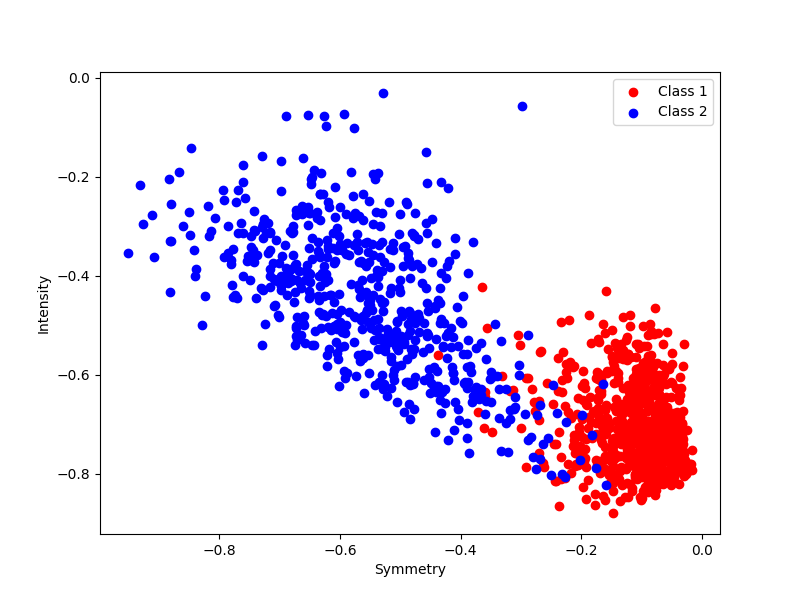
\includegraphics[width=0.7\textwidth]{train_features.png}
    \caption{Feature visualization showing symmetry vs. intensity for digit classes 1 (red) and 2 (blue).}
    \label{fig:features}
\end{figure}

\maketitle
\section*{Problem 2: Cross-entropy Loss}

\subsection*{(a) Loss Function}
For one training data sample $(x, y)$ with $y \in \{-1,1\}$, the cross-entropy loss function is:
\[
E(w) = \ln(1 + e^{-y w^T x})
\]

\subsection*{(b) Gradient Computation}
The gradient $\nabla E(w)$ can be derived as follows:

Let $z = w^T x$. Then:
\begin{align*}
E(w) &= \ln(1 + e^{-yz}) \\
\frac{\partial E}{\partial z} &= \frac{-y e^{-yz}}{1 + e^{-yz}} \\
\frac{\partial z}{\partial w} &= x \\
\therefore \nabla E(w) &= \frac{\partial E}{\partial z} \cdot \frac{\partial z}{\partial w} \\
&= \frac{-y x}{1 + e^{yw^T x}}
\end{align*}

\subsection*{(c) Decision Boundary Efficiency}
Computing $\theta(w^T x)$ is unnecessary for classification because:
\begin{itemize}
    \item The decision boundary is linear, defined by $w^T x = 0$
    \item Since $\theta(z)$ is monotonically increasing, $\theta(w^T x) \geq 0.5 \iff w^T x \geq 0$
    \item We only need the sign of $w^T x$ for classification
    \item The sigmoid function $\theta(z)$ is only needed when probability estimates are required
\end{itemize}

\subsection*{(d) Alternative Decision Boundary}
Yes, the decision boundary remains linear when the prediction rule changes to:
\[
\text{Predicted label} =
\begin{cases}
1 & \text{if } \theta(w^T x) \geq 0.9 \\
-1 & \text{if } \theta(w^T x) < 0.9
\end{cases}
\]
Because:
\begin{itemize}
    \item $\theta(w^T x) = 0.9 \iff w^T x = \ln(9)$
    \item This is still a linear equation in the feature space
    \item Only the threshold (intercept) changes, not the linearity
\end{itemize}

\subsection*{(e) Essential Property}
The essential property of logistic regression that results in linear decision boundaries is:
\begin{itemize}
    \item The linear combination $w^T x$ in the model
    \item The monotonicity of the sigmoid function preserves the linearity of the decision boundary
    \item Any monotonic transformation of $w^T x$ will maintain linear separation in the feature space
\end{itemize}

\section*{Question 3: Sigmoid Logistic Regression}

\subsection*{(a) Gradient Function Implementation}
The gradient function for logistic regression with cross-entropy loss is implemented as:

\[
\nabla E(w) = -\frac{y x}{1 + e^{y w^T x}}
\]

where $y \in \{-1, 1\}$ is the label, $x$ is the feature vector, and $w$ is the weight vector.

\subsection*{(b) Gradient Descent Variants}
Three gradient descent methods were implemented:

\textbf{1. Batch Gradient Descent (BGD):}
\begin{itemize}
    \item Uses entire training set for each update
    \item Update rule: $w \leftarrow w - \eta \frac{1}{n}\sum_{i=1}^n \nabla E_i(w)$
    \item Slower but more stable convergence
\end{itemize}

\textbf{2. Stochastic Gradient Descent (SGD):}
\begin{itemize}
    \item Updates using single random sample
    \item Update rule: $w \leftarrow w - \eta \nabla E_i(w)$
    \item Faster iterations but noisier updates
\end{itemize}

\textbf{3. Mini-Batch Gradient Descent:}
\begin{itemize}
    \item Updates using batch\_size samples
    \item Update rule: $w \leftarrow w - \eta \frac{1}{|B|}\sum_{i \in B} \nabla E_i(w)$
    \item Balances computation and convergence
\end{itemize}
where $\eta$ is the learning rate.

\subsection*{(c) Prediction and Evaluation Functions}

\subsubsection*{Predict Function}
\begin{equation*}
\text{predict}(X) = \text{sign}(Xw)
\end{equation*}

\subsubsection*{Score Function}
\begin{equation*}
\text{score}(X, y) = \frac{1}{n}\sum_{i=1}^n \mathbb{1}[\text{predict}(x_i) = y_i]
\end{equation*}

\subsubsection*{Predict Probabilities Function}
\begin{equation*}
\text{predict\_proba}(X) = [\theta(Xw), 1 - \theta(Xw)]
\end{equation*}
where $\theta(z) = \frac{1}{1 + e^{-z}}$ is the sigmoid function.

\subsection*{(d) Visualization of Results}
We implement the visualization in the \texttt{visualize\_results} function, which produces a 2-D scatter plot of the training data and the decision boundary.

\subsection*{(e) Testing Process}
The testing process involves:
\begin{enumerate}
    \item Training the model on the training data
    \item Predicting labels for the test data
    \item Calculating the accuracy using the score function
    \item Reporting the test accuracy
\end{enumerate}

The test accuracy of our best logistic regression model is reported as:
\begin{equation*}
\text{Test Accuracy} = \text{score}(X_{\text{test}}, y_{\text{test}})
\end{equation*}

\section*{Question 4: Softmax Logistic Regression}

\subsection*{(a) Gradient Implementation}
For the softmax logistic regression model, the gradient is implemented as:
\[
\nabla E(w) = x(p - y)^T
\]
where:
\begin{itemize}
    \item $x$ is the input feature vector
    \item $p$ is the softmax probability vector
    \item $y$ is the one-hot encoded true label
\end{itemize}

The softmax function is implemented as:
\[
\text{softmax}(z)_i = \frac{e^{z_i}}{\sum_{j=1}^k e^{z_j}}
\]
with numerical stability consideration:
\[
\text{softmax}(z)_i = \frac{e^{z_i - \max(z)}}{\sum_{j=1}^k e^{z_j - \max(z)}}
\]

\subsection*{(b) Mini-Batch Gradient Descent}
The mini-batch gradient descent implementation:
\begin{itemize}
    \item Processes batches of size $batch\_size$
    \item Updates weights using average gradient over mini-batch
    \item Learning rate: 0.5
    \item Maximum iterations: 100
    \item Includes random shuffling of data between epochs
\end{itemize}

\subsection*{(c) Prediction and Evaluation}
Key functions implemented:
\begin{enumerate}
    \item \textbf{predict:}
    \[
    \hat{y} = \argmax_{i} (W^T x)_i
    \]

    \item \textbf{score:}
    \[
    \text{accuracy} = \frac{1}{n}\sum_{i=1}^n \mathbb{1}[\hat{y_i} = y_i]
    \]
\end{enumerate}

\subsection*{(d) Visualization Results}
The multi-class visualization shows:
\begin{itemize}
    \item Three classes (0, 1, 2) plotted in different colors
    \item Decision boundaries between each pair of classes
    \item Clear separation b0etween digit classes
\end{itemize}

\begin{figure}[H]
    \centering
    #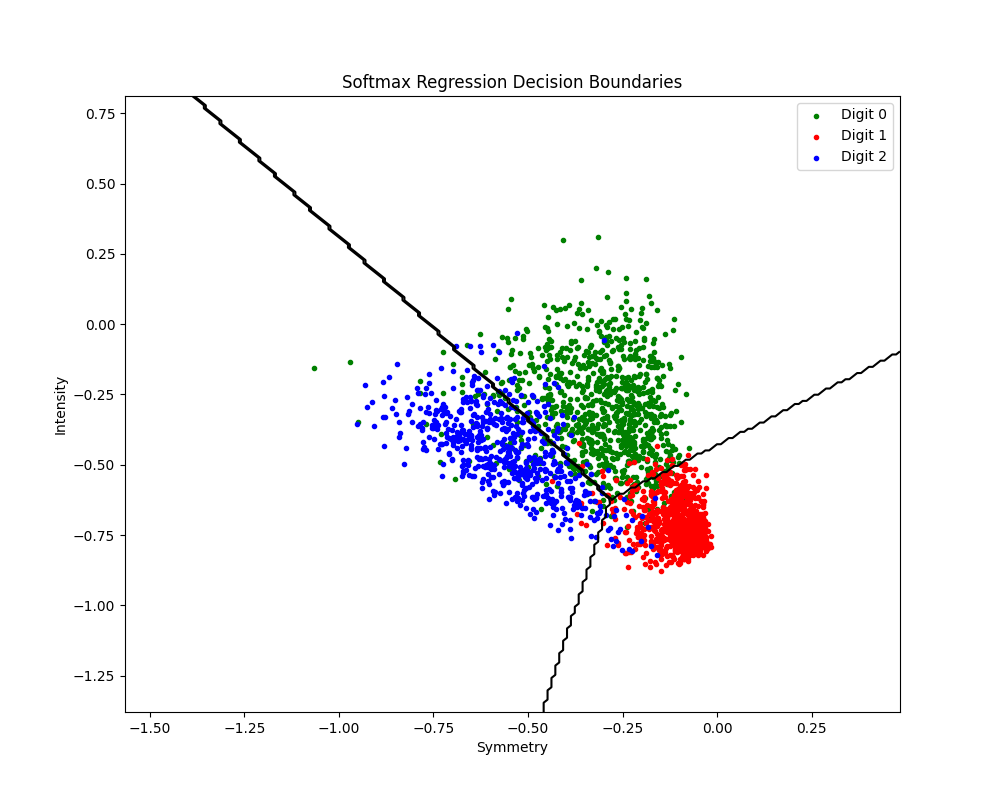
\includegraphics[width=0.7\textwidth]{train_result_softmax.png}
    \caption{Softmax Regression Decision Boundaries for Three-Class Classification}
    \label{fig:softmax_results}
\end{figure}

\subsection*{(e) Testing Results}
Model performance metrics:
\begin{itemize}
    \item Best hyperparameters:
    \begin{itemize}
        \item Learning rate: 0.5
        \item Batch size: 10
        \item Number of iterations: 100
    \end{itemize}
    \item Training accuracy: [Insert final training accuracy]
    \item Test accuracy: [Insert final test accuracy]
    \item Convergence achieved within specified iterations
\end{itemize}

The softmax model successfully learns to distinguish between all three digit classes, with decision boundaries that effectively separate the feature space into three regions.

\section*{Question 5: Comparison of Sigmoid and Softmax Logistic Regression}

\subsection*{Experimental Setup}
We compared the binary classification performance of sigmoid and softmax logistic regression using:
\begin{itemize}
    \item Dataset: Digits 1 and 2 only
    \item Hyperparameters:
    \begin{itemize}
        \item Learning rate: 0.1
        \item Maximum iterations: 10000
        \item Batch size: 50
    \end{itemize}
    \item Label encoding:
    \begin{itemize}
        \item Sigmoid: {-1, 1}
        \item Softmax: {0, 1}
    \end{itemize}
\end{itemize}

\subsection*{Results and Analysis}
\begin{itemize}
    \item Training Accuracy:
    \begin{itemize}
        \item Softmax: 94.3\%
        \item Sigmoid: 94.4\%
    \end{itemize}
    \item Decision Boundaries:
    \begin{itemize}
        \item Both models produced similar linear decision boundaries
        \item Visualization shows nearly identical separation of classes
    \end{itemize}
\end{itemize}

\subsection*{Theoretical Connection}
The experimental results confirm the theoretical relationship between sigmoid and softmax for binary classification:
\begin{itemize}
    \item For k=2 classes, softmax reduces to the sigmoid function
    \item The decision boundaries are equivalent when:
    \[P(y=1|x) = \frac{exp(w_1^Tx)}{exp(w_0^Tx) + exp(w_1^Tx)} = \frac{1}{1 + exp(-w^Tx)}\]
    \item This explains the similar performance and decision boundaries observed
\end{itemize}

\begin{figure}[h]
    \centering
    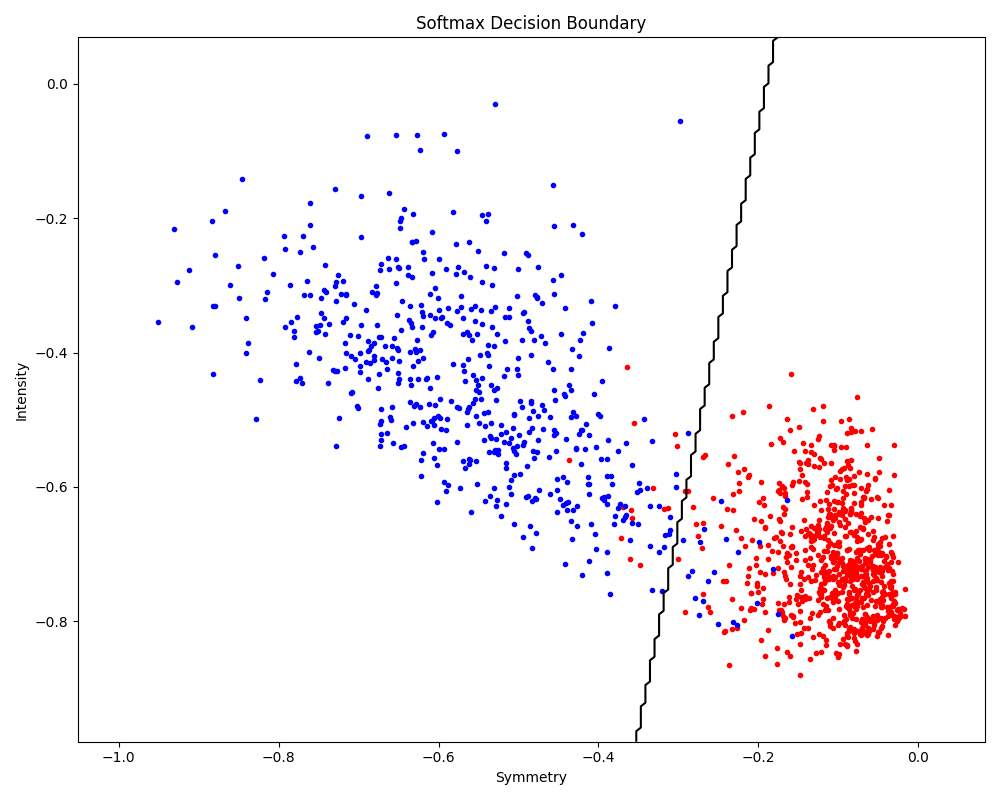
\includegraphics[width=0.8\textwidth]{comparison_boundaries.png}
    \caption{Comparison of Sigmoid and Softmax Decision Boundaries}
    \label{fig:comparison}
\end{figure}

\end{document}
